\chapter{Testy}
\label{cha:testy}

Sterowanie za pomocą komend głosowych może stać się o wiele cięższe w wykonaniu, kiedy w grę wchodzą czynniki takie jak akcent, inny niż stosowany w algorytmie język, dźwięki w tle, złożoność polecenia czy nawet niewyraźna mowa. Z uwagi na ten fakt, algorytm do rozpoznawania mowy używany w programie został poddany scenariuszom testowym. 

Na potrzeby testów stworzono pięć zestawów tych samych dziesięciu poleceń, różniących się pomiędzy sobą kilkoma czynnikami:
\begin{itemize}
    \item oryginalny zestaw komend w języku angielskim z akcentem amerykańskim \textit{[EN]},
    \item wersja w języku angielskim z akcentem amerykańskim, gdzie prędkość nagrania to 2.0 \textit{[EN-0-2]},
    \item wersja w języku angielskim z akcentem Indii \textit{[EN-IN]},
    \item wersja w języku angielskim z akcentem Hong Kongu, gdzie prędkość nagrania to 0.5, a tonacja wyższa o 20 od normalnej \textit{[EN-HK-20-05]},
    \item wersja w języku polskim \textit{[PL]}.
\end{itemize}

Do zestawów danych została dołożona również wersja polska, celem sprawdzenia użyteczności algorytmu w wypadku implementacji na fizycznym urządzeniu. Modyfikacje prędkości, tonacji i akcentów zostały wykonane na potrzeby zróżnicowania danych i wprowadzenia trudności dla algorytmu do zrozumienia komend. 

Używając metryki WER \ref{eq:wer} została obliczona średnia wartość błędu w skali od 0 do 1 dla każdego z zestawów danych, widoczna na wykresie \ref{fig:dts1}. Można na nim zauważyć, że zgodnie z oczekiwaniami, zestaw \textit{[EN]} oryginalnych komend w języku angielskim posiada najmniejszą wartość błędu. Zarówno zestaw z akcentem Indii \textit{[EN-IN]} jak ten z akcentem Hong Kongu radzą sobie równie dobrze. Najbardziej wyróżnia się zestaw komend po polsku \textit{[PL]}, ze względu na niewystępujące w transkrypcji znaki łacińskie.

\begin{center}
    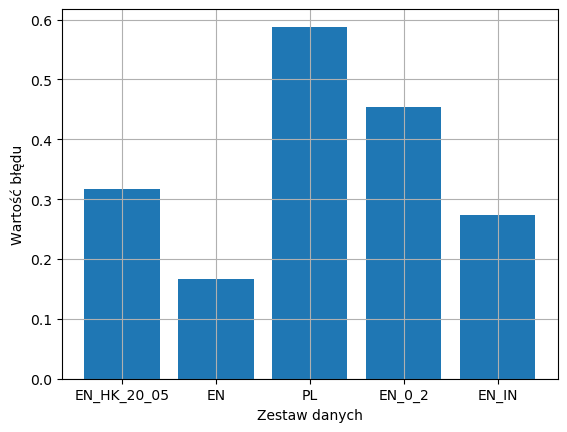
\includegraphics[width=0.7\linewidth]{files/output1.png}
    \captionof{figure}{Średnia wartość błędu}
    \label{fig:dts1}
\end{center}

Po uwzględnieniu w transkrypcji znaków łacińskich, można zauważyć na wykresie \ref{fig:dts2} znaczny spadek wartości błędu dla zestawu komend w języku polskim. Potwierdza to użyteczność wykorzystywanego algorytmu do rozpoznawania mowy również poza środowiskiem testowym.

\begin{center}
    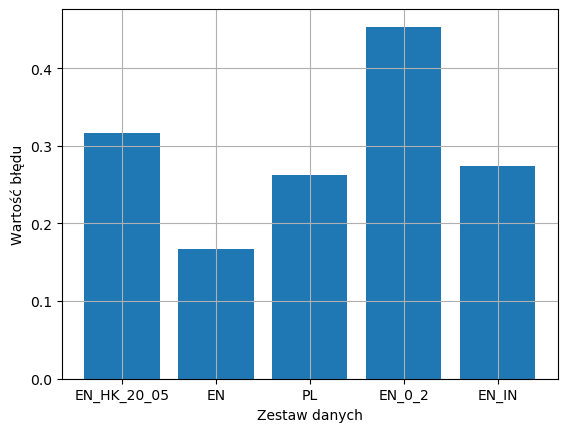
\includegraphics[width=0.7\linewidth]{files/output2.png}
    \captionof{figure}{Średnia wartość błędu po uwzględnieniu znaków łacińskich}
    \label{fig:dts2}
\end{center}

Dane w zestawach dzielą się na dwie kategorie pod względem długości polecenia:
\begin{itemize}
    \item proste komendy poniżej 15 znaków \textit{[słowa krótkie]},
    \item bardziej złożone komendy powyżej 15 znaków \textit{[słowa długie]}.
\end{itemize}

% dopisz tu cos TODO
% czy dodawac reference  do stronki konwertera

\begin{center}
    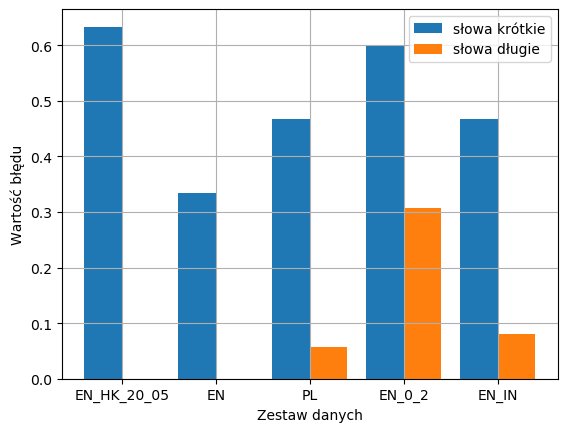
\includegraphics[width=0.7\linewidth]{files/output3.png}
    \captionof{figure}{Średnia wartość błędu dla słów krótkich i słów długich}
    \label{fig:dts3}
\end{center}

%  jeszcze wykres x to slowa y to srednie rozpoznawanie ich? - nwm zobacze rano
% analiza tych zestawow danych, gdzie jest modyfikacja - WAZNE
% tutaj jeszcze mozna wrzucic testy samego robota - nie wiem jeszcze jak

% Scenariusze testowe:
% 1. inny akcent niz eng-us - indi
% 1. mowa po polsku - czy w ogole rozpoznaje język?
% 2. złożone komendy
% 3. muzyka np w tle/bardzo cicho
% chin - pitch -20, speed -0.5
% indi - speed 2.0

%---------------------------------------------------------------------------